%----------------------------------------------------------------------------------------
%	PACKAGES AND OTHER DOCUMENT CONFIGURATIONS
%----------------------------------------------------------------------------------------

\documentclass[12pt]{article} % Default font size is 12pt, it can be changed here
% Margin specification
% Check http://en.wikibooks.org/wiki/LaTeX/Page_Layout for more info
\usepackage[margin = 1in]{geometry}
\usepackage[nottoc,notlof,notlot,numbib]{tocbibind}

% Some misc and math packages
% Check http://en.wikibooks.org/wiki/LaTeX/Mathematics for more info
\usepackage{fancyhdr}
\usepackage{manfnt}
\usepackage{pgf}
\usepackage{amsmath,amsthm,amssymb,natbib,graphicx}
\usepackage{amsfonts}
\DeclareMathAlphabet{\mathpzc}{OT1}{pzc}{m}{it}
\usepackage{bbm}
\usepackage{float}
\usepackage{mathrsfs} %mathscr{A}
\usepackage{hyperref}
\usepackage{pdfpages}

% Color
\usepackage{color}

% For specifying the counter style of enumerate
\usepackage{enumerate}

\usepackage{geometry} % Required to change the page size to A4
%\geometry{a4paper} % Set the page size to be A4 as opposed to the default US Letter

\usepackage{graphicx} % Required for including pictures

\usepackage{float} % Allows putting an [H] in \begin{figure} to specify the exact location of the figure
\usepackage{wrapfig} % Allows in-line images such as the example fish picture

\usepackage{parskip} % Space between paragraphs

\usepackage{lipsum} % Used for inserting dummy 'Lorem ipsum' text into the template

\linespread{1.0} % Line spacing

\setlength\parindent{0pt} % Uncomment to remove all indentation from paragraphs

\graphicspath{{./Pictures/}} % Specifies the directory where pictures are stored

\newcommand{\iid}{\stackrel{\mathrm{iid}}{\sim}}

% Page style definition
\rfoot{\today}
\begin{document}


%------------------------------------------------
\begin{titlepage}

\newcommand{\HRule}{\rule{\linewidth}{0.5mm}} % Defines a new command for the horizontal lines, change thickness here

\center % Center everything on the page
 
%----------------------------------------------------------------------------------------
%	HEADING SECTIONS
%----------------------------------------------------------------------------------------

\textsc{\LARGE Johns Hopkins University}\\[1.5cm] % Name of your university/college
\textsc{\Large Computational Genomics}\\[0.5cm] % Major heading such as course name
\textsc{\large EN 600.639}\\[0.5cm] % Minor heading such as course title

%----------------------------------------------------------------------------------------
%	TITLE SECTION
%----------------------------------------------------------------------------------------

\HRule \\[0.4cm]
{ \huge \bfseries Augmenting Phylogenetic Classification of Metagenomic Reads}\\[0.4cm] % Title of your document
\HRule \\[1.5cm]
 
%----------------------------------------------------------------------------------------
%	AUTHOR SECTION
%----------------------------------------------------------------------------------------

\begin{minipage}{0.4\textwidth}
\begin{flushleft} \large
\emph{Authors:}\\
Shuya \textsc{Chu}, \\  Stephen \textsc{Cristiano}, \\ Bing \textsc{He},\\  Zhou \textsc{Ye} % Your name
\end{flushleft}
\end{minipage}
~
\begin{minipage}{0.4\textwidth}
\begin{flushright} \large
\emph{Instructor:} \\
Dr. Ben \textsc{Langmead} % Supervisor's Name
\end{flushright}
\end{minipage}\\[4cm]

% If you don't want a supervisor, uncomment the two lines below and remove the section above
%\Large \emph{Author:}\\
%John \textsc{Smith}\\[3cm] % Your name

%----------------------------------------------------------------------------------------
%	DATE SECTION
%----------------------------------------------------------------------------------------

{\large \today}\\[3cm] % Date, change the \today to a set date if you want to be precise

%----------------------------------------------------------------------------------------
%	LOGO SECTION
%----------------------------------------------------------------------------------------

%\includegraphics{Logo}\\[1cm] % Include a department/university logo - this will require the graphicx package
 
%----------------------------------------------------------------------------------------

\vfill % Fill the rest of the page with whitespace
 \end{titlepage}
%------------------------------------------------
\vspace{5 ex}
\begin{abstract}
In recent years, metagenomics has gained increased interest in the scientific community. With relevance to  public health, agriculture, biofuels, and marine biology [\cite{Wooley:2010dg}], it is important to understand the taxonomic composition of metagenomic samples and its functional impact it their respective ecosystems. In this project, we use simulated data to explore a variety of methods to taxonomically classify metagenomic reads to their correct position in a phylogenetic reference set. In particular, we use three methods: bloom filter, bowtie, interpolated Markov model and we find bloom filter and bowtie have high accuracy for classifying metagenomics reads to our reference genomes. 
\end{abstract}

\section{Introduction}
The recent expansion of next generation sequencing technologies have greatly benefited our ability to study microbial communities. Metagenomics, defined in 2005 as ``The application of modern genomics techniques to the study of communities of microbial organisms directly in their natural environments, bypassing the need for isolation and lab cultivation of individual species'' [\cite{Chen:2005dg}], has seen a surge of research efforts in recent years in diverse fields including public health, agriculture, biofuels, and marine biology, and efforts such as the Human Microbiome Project generating large quantities of metagenomic data. Despite this, computational methods are still needed for analyzing and making sense of these data in an accurate but efficient matter. 
\par
One important challenge is, given a set of metagenomic reads, to accurately classify the taxonomic composition of the reads. For example, a metagenomic human gut sample will contain many different microbial species. We wish to be able to classify each read to the correct phylogenetic location in a reference set and determine the presence and abundance of different microbial species in the sample. Adding to the challenge, many of the species will be closely related (belonging to the same genus, family etc) and in a microbial sample, many of the reads make come from \emph{de novo} genomes, \emph{i.e.} from species that have never been sequenced before and unknown to the scientific community. 
\par
In this project, we propose, implement, and compare three methods for the classification of metagenomic reads. In particular, we provide a Bloom filter approach, an approach based on Interpolated Markov Models, and an approach based using Bowtie to perform local alignment to reference genomes and classify using a novel algorithm. While similar methods exist, we also consider a number of ways in which we can improve upon these.
\par
To perform our analyses, we obtain reference genomes from RefSeq, a large collection of genomes maintained by the National Center for Biotechnology Institute (NCBI) [\cite{Pruitt:2009dg}] 
\section{Related work}
A large body of work has already been done on the phylogenetic classification of metagenomic reads. It's important to note that many of the early methods are only accurate for large sequence reads and fail at correctly classifying the short ($ \sim100$ bp) reads generated by next generation sequencers [\cite{Brady:2009dg}]. We briefly review a few of the more recent metagenomic classification methods.
\subsection{PhymmBL}
PhymmBL [\cite{Brady:2009dg}] uses an Interpolated Markov Model to phylogenetically classify genomic reads to genomes in RefSeq, a large collection of genomes. It is capable of performing classification at different levels of the phylogentic tree (species, genus, family etc). In addition to classification using an IMM, PhymmBL also uses BLAST for local alignment to classify. By applying a linear function of the scores from the IMM and BLAST, the authors report greater classification accuracy than either the IMM or BLAST alone. Though very accurate, PhymmBL suffers from extremely slow running time, due to using BLAST for local alignment. 

\subsection{FACS}
Fast Accurate Classification of Sequences (FACS) [\cite{Stranneheim:2010dg}] transforms the reference genomes to Bloom filters and query Bloom filters for exact matches. Bloom filters are an compact hash-based data structure which are used to quickly determine whether an element is a member of a set or not. In a trade-off for compactness and speed of look-up, Bloom filters come with a risk of giving false positives which must be controlled. FACS is implemented in PERL and achieves high speed, but is limited to using Bloom filters $<312 MB$ and does not have a scoring system optimized for classification. In a comparison of classification software, other authors have reported an inability to reproduce the results reported in the FACS paper [\cite{Bazinet:2012dg}].

\subsection{Bowtie}
Bowtie [\cite{Langmead:2009dg}] utilizes a Burrow-Wheeler Transform and an FM index to perform extremely fast alignment of short DNA reads to a reference genome. By performing local alignment of the reads to each of the reference genomes from a phylogenetic tree, and using an appropriate scoring system, Bowtie can be adapted for classification of metagenomic reads. 

\section{Methods and software}
We obtain our reference genomes from RefSeq, obtained from the NCBI. Due to the vast size of RefSeq, we initially considered only the phylum \emph{Proteobacterium}, but even that exceeded our memory limits. For this reason, we decided to use comparisons of the methods for our reference set the genomes from \emph{Escherichia coli} (strain K-12 substain. DH10B) and  \emph{Bdellovibrio bacteriovorus}. To simulate our data, we use the software MetaSim [\cite{Richter:2008dg}] which will generate metagenomic reads into a FASTA file given a set of reference genomes.
\par
As the main purpose of the Bowtie method was to develop an algorithm that will not have align to every genome in a reference set, we also considered 15 genomes from \emph{Proteobacterium} but the same simulated reads. However, the comparisons with the other methods were still conducted only on the two previously mentioned reference genomes.

\subsection{Bloom Filter augmented Classification (BFAC)}
In this section, we describe the Bloom Filter augmented Classification (BFAC) method. In a nutshell, BFAC is a bloom filter based classification methods for metagenomic phylogenetic classification. Currently the only relevant work we can find is the FACS methods [\cite{Stranneheim:2010dg}]. FACS methods can classify metagenomic sequences as belonging or not belonging to a reference sequence. To fulfill this goal, FACS counted the matched k-mers of a query sequence and set a threshold to make a dichotomized classification. Our BFAC method augmented FACS to be applicable in the situation of metagenomic phylogenetic classification. There are two major augmentations. First, in addition to dichotomized classification scheme as implemented in FACS, BFAC can not only make multi-category classification but also perform phylogenetic classification. More specifically, when species-level classification fails for a query sequence, BFAC will automatically classify the sequence to higher level (e.g., genus level) based on an entropy-based summary statistics based on the species-level scores. Second, BFAC speeds up the querying process by a two-step scan system: a coarse scanning and a detailed scanning. 
\par
In BFAC, we first build a bloom filter for the reference genomes of species in our selected subtree of the NCBI taxonomy. Each reference genome is decomposed into k-mers with a specified length; those k-mers are then inserted into the initialized Bloom Filter as keys. In order to fully take advantage of the Bloom Filter data structure, we initialize a differently-sized bloom filter for different reference genome based on genome sizes and total number of k-mers. When initializing the bloom filter, we also specify the acceptable false positive rate. As it is shown in previous study [\cite{Broder:2004dg}], the size of the bitmap grows linearly with the number of elements in the bitmap. Note that we explore how the specified k-mer length and false positive rate would affect our classification accuracy and time used to query (please refer to relevant figures in the result section). Second, once the filters are built, we can interrogate them with multiple metagenomic reads and record the match scores. More specifically, metagenomic reads are decomposed into k-mers with the same length and are used ask keys for querying bloom filters. Third, we perform the phylogenetic classification of each reads and output the results. We implemented the BFAC in perl using perl module BLOOM::FASTER based on the FACS code. 
\par
There are two things we tried for which we didn’t present results here. The first thing is to incorporate false positive rate of bloom filter into the scoring system. We penalized the scores according to the uncertainty implied by the false positive rate of the bloom filter. We didn’t present the results because we found that the classification accuracy change very little when we use different false positive rate (from 0.0005 to 0.0035, please refer to figures in results section). The second thing we tried is to use a variant of classic bloom filter for our BFAC. We explored scalable bloom filters that can dynamically adapt to the stored keys while keeping an acceptable false positive rate; and the attenuated bloom filters with a depth large than 1 to store the set of species under the same genus instead of building a  bloom filter for each reference genome. We came across some technical problems and didn’t have enough time to complete, so we did not present the results here.

\subsection{Improvement with Bowtie2}
Bowtie2 is an ultrafast aligner using FM index. It is particularly good at aligning reads of about 50 up to 100s or 1,000s of characters. Since our simulate testing data is around 100-200 long, using Bowtie2 will lead to fast aligning.
\par
The idea for improvement is by skipping some unnecessary alignment between the test data and reference, identifying the species for test data will be much more fast. Like what we did in the Boyer-Moore method in class, we use results from comparisons to skip future alignments that definitely won't match. To be more specific,  if we got a really low score when aligning the test data with one species, it means the sample is definitely not from this species, thus we can skip the whole species from the same genus. For example, if we know this sample definitely does not belong to \emph{Canis}, instead of checking whether it's \emph{Canis lupus}, we can check whether it's \emph{Cuon alpinus} from the genus of \emph{Cuon}.
\par
First we construct a tree structure to describe the taxonomy relation between the reference in python. For each node, node.data represent directory path of this reference, parent and children is directory path for its parent and children in the reference subtree we used. 
\par
Then by running Bowtie2, we will have scores which describe the similarity between the sample data and reference. If scores is really low, in other words, we have enough confidence to say the sample is not from this species, we skip the whole genus this reference species belongs to. If scores is not that bad, we will go through all the species in this genus to determine which species it has most similarity with.  
\par
Threshold here is very important. We didn't come up with a fixed expression to calculate it by the due date. We extract 31 species from 18 genus from the reference set and set the threshold after observing the result from those alignments. Also, we used the average score from the scores of 1000 test sequence in the .fna file.
\par
In order to run the code, please change the value of 'projectpath' to the actual path that 'Bowtie.tar.gz' you extract to. And also, make sure inside the 'projectpath', there is a /data/index folder and a /bowtie2-2.1.0 folder.

\subsection{Interpolated Markov Model}
DNA sequence can be represented by a sequence of random variables $X_1, X_2, \cdots, X_n$ where $X_i$ is the base at position $i$ which can take a value from $(A, T, C, G)$. Markov model assumes the probability of $X_i$ taking on some value will depend on $X_{i-1}, X_{i-2}, \cdots, X_{i-n}$. $n$ is the number of order which shows how many bases we need to predict $X_i$. In this way, any DNA sequence can be scored by computing the probability for different position generated by Markov model. 
\par
There is a trade-off in Markov model. For an n-th order Markov model, the parameters to estimate on one position for a fixed-length DNA sequence is $4^{n+1}$. If we use low-order Markov model, there are fewer parameters but less prediction power. However, if we use high-order Markov model, we will obtain strong prediction power but the parameters will be exponentially large. It is very likely that there are insufficient data to learn the parameters. 
\par
Interpolated Markov model (IMM) successfully combines the merits of low-order and high-order models by using a linear combination of Markov models. The idea is generally from Salzberg's paper[\cite{Salzberg:1998dg}]. All the mathematics are in the appendix and we think the threshold in the original paper for $\xi^2$-test $0.5$ is incorrect. The confidence score i.e. the p-value should be smaller than $0.05$. Correct us if you think we are not right. 
\par
We implement IMM all by ourselves using Java and the speed is very good. We have tried our best to minimize the times of scanning data set. I also do something Salzberg did not do in his paper, which is show the effect of order and threshold. 

The general steps we follow to implement IMM are:

\begin{enumerate}
\item Training the parameters of IMM from reference genomes;
\item Use the parameters of each reference genome to score the test genomes;
\item Label the test genomes with the reference genomes which have highest score;
\end{enumerate}

Here we do something a little different. After getting the score, we use a second threshold to screen the score. We call it score standard. When the score is too low (below threshold), we treat the test genome unclassified; otherwise, we use the same tool to label the test genome. 

\section{Results}
\subsection{Evaluation Method}
We compute five statistics to do the comparison in this paper. They are classification accuracy, sensitivity of B, specificity of B, sensitivity of E and specificity of E where B is Bdellovibrio bacteriovorus and E is Escherichia Coli. We use "B" and "E" to notate two bacteria for the entire paper. The formula to compute them are as following:

\begin{table}
\centering
\begin{tabular}{|c|c|c|}
\hline
 & E & B \\
 \hline
 E & EE & EB \\
 \hline
 B & BE & BB \\
 \hline
 N & NE & NB \\
 \hline
\end{tabular}
\end{table}
where $EE, EB, BE, BB, NE, NB$ are counts. Here $N$ means we neither classify the test genome B not E. 

\begin{equation}
\begin{aligned}
&Acc = \frac{EE+BB}{EE+EB+BE+BB+NE+NB}\\
&Sen(B) = \frac{BB}{BB+EB+NB}\\
&Spe(B) = \frac{NE+EE}{EE+NE+BE}\\
&Sen(B) = \frac{EE}{EE+BE+NE}\\
&Spe(B) = \frac{BB+NB}{EB+BB+NB}
\end{aligned}
\end{equation}

\subsection{All Results}
\begin{figure}
\centering
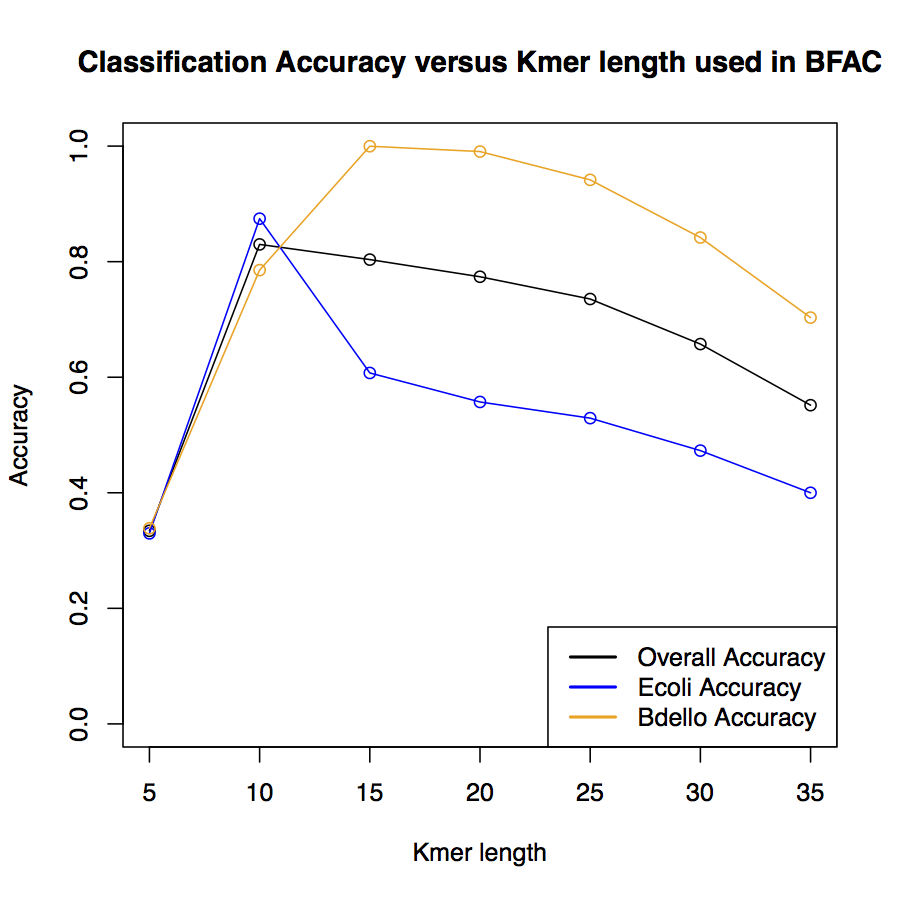
\includegraphics[width=0.8\textwidth]{KmerLength.png}
\caption{Classification accuracy versus Kmer length used in BFAC}
\label{fig: kmer}
\end{figure}

\begin{figure}
\centering
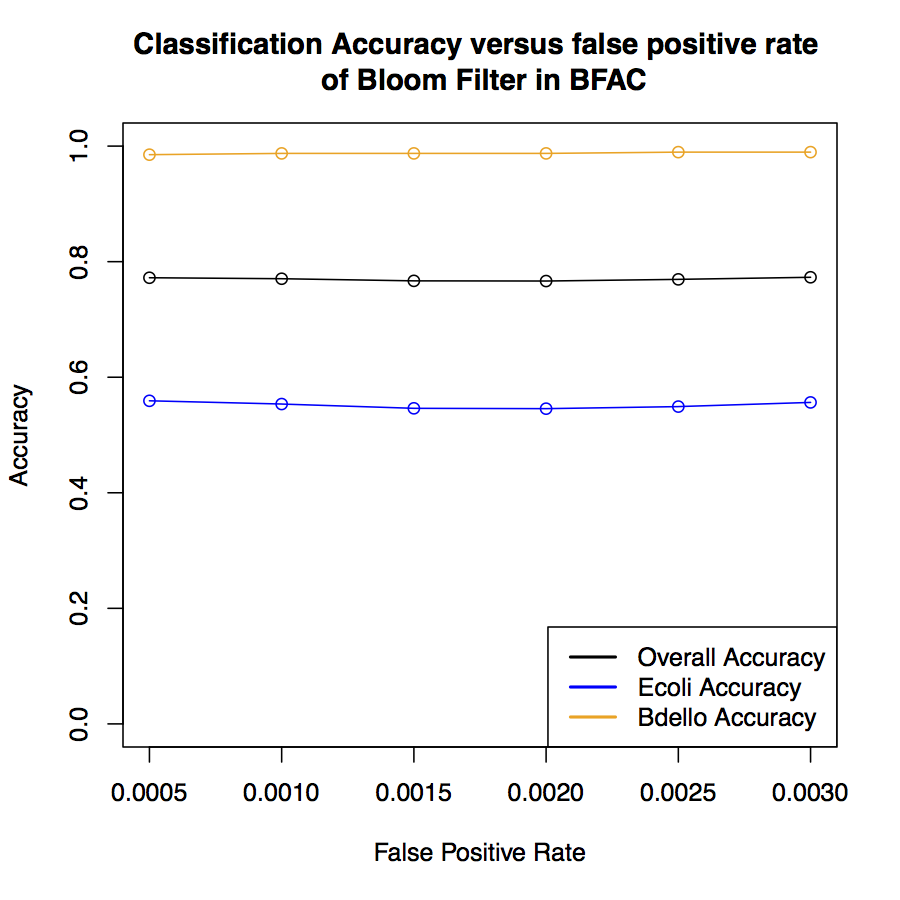
\includegraphics[width=0.8\textwidth]{FlaseDiscoveryRate.png}
\caption{Classification accuracy versus false positive rate of bloom filter in BFAC}
\label{fig: false}
\end{figure}

\begin{table}
\centering
\begin{tabular}{|c|c|}
\hline
Method & Time \\
\hline
Skip & 6.3978 \\
\hline
No Skip & 12.2367 \\
\hline
\end{tabular}
\label{tab: bowtie}
\caption{Bowtie Comparison}
\end{table}

\begin{table}
\centering
\begin{tabular}{|c|c|c|c|c|c|}
\hline
Order & Accuracy & Sens(B) & Spec(B) & Sens(E) &  Spec(E) \\
\hline
2 & 0.4781 & 0.023 & 0.943 & 0.9332 & 0.026 \\
\hline
4 & 0.4626 & 0.1816 & 0.7478 & 0.7436 & 0.1826 \\
\hline
6 & 0.4975 & 0.0014 & 0.9966 & 0.9936 & 0.0018 \\
\hline
8 & 0.3341 & 0 & 1 & 0.6682 & 0.1912 \\
\hline
10 & 0.3341 & 0 & 1 & 0.6682 & 0.1912 \\
\hline
\end{tabular}
\caption{Comparison For Different Orders}
\label{tab: order}
\end{table}

\begin{table}
\centering
\begin{tabular}{|c|c|c|c|c|c|}
\hline
Threshold & Accuracy & Sens(B) & Spec(B) & Sens(E) &  Spec(E) \\
\hline
200 & 0.2054 & 0 & 1 & 0.4108 & 0.4338 \\
\hline
300 & 0 & 0 & 1 & 0 & 0.9998 \\
\hline
400 & 0.4975 & 0.0014 & 0.9966 & 0.9936 & 0.0018 \\
\hline
500 & 0.0204 & 4.00E-04 & 0.9994 & 0.0404 & 0.9296 \\
\hline
600 & 0.2087 & 0.0066 & 0.9838 & 0.4108 & 0.4338 \\
\hline
\end{tabular}
\caption{Comparison For Different Thresholds}
\label{tab: threshold}
\end{table}

\begin{table}
\centering
\begin{tabular}{|c|c|c|c|c|c|}
\hline
Standard & Accuracy & Sens(B) & Spec(B) & Sens(E) &  Spec(E) \\
\hline
50 & 0.4977 & 0.0018 & 0.9936 & 0.9936 & 0.0018 \\
\hline
60 & 0.4975 & 0.0014 & 0.9966 & 0.9936 & 0.0018 \\
\hline
70 & 0.233 & 0 & 1 & 0.466 & 0.365 \\
\hline
80 & 0.0042 & 0 & 1 & 0.0084 & 0.9826 \\
\hline
90 & 0 & 1 & 1 & 0 & 0.9996 \\
\hline
\end{tabular}
\caption{Comparison For Different Score Standards}
\label{tab: standard}
\end{table}

\begin{figure}
\centering
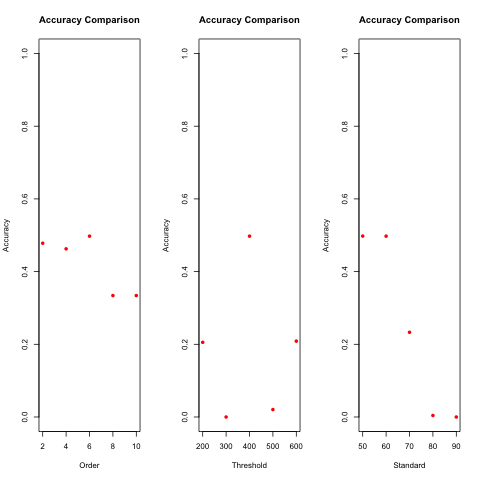
\includegraphics[width=0.8\textwidth]{all.png}
\caption{All Comparison}
\label{fig: all}
\end{figure}

\begin{table}
\begin{tabular}{|c|c|c|c|c|c|c|}
\hline
Method & Accuracy & Sens(B) & Spes(B) & Sens(E) & Spes(E) & Time(s) \\
\hline
Bowtie & 0.9649 & 0.9298 & 1 & 1 & 0.9702 & 12 \\
\hline
Bloom Filter & 0.8036 & 0.6074 & 0.5 & 0.9998 & 0.5 & 52 \\
\hline
IMM & 0.4975 & 0.0014 & 0.9966 & 0.9936 & 0.0018 & 14 \\
\hline
\end{tabular}
\caption{Comparison of All Methods}
\label{tab: all_comp}
\end{table}

\section{Discussion}

\subsection{Bloom Filter augmented Classification (BFAC)}
The figure \ref{fig: kmer} shows how the classification accuracies change in response to the specified Kmer length when build the bloom filter. As we can see from the figure, the classification accuracy for Bdello and Ecoli as well as the overall accuracy are quite low when the kmer length is 5. This is reasonable as short kmers can occur frequently in different reference genomes as they are not specific enough for capturing the source of metagenomic reads. The accuracies increase as the kmer length increase to around 15 bp and decrease as the kmer length further increase to 35. This is probably due to the fact that longer kmer is more likely to contain errors and become harder to get classified. Based on the figure the optimal length of kmer to be used is between 10-15 bp. We think that this number is generally applicable to bacteria. Note that the time for building bloom filter and the bitmap sizes also change in response to the length of k-mers used.

The figure \ref{fig: false} presents how the classification accuracies change with regard to false positive rate used to build bloom filter in BFAC. Surprisingly, the Bdello and Ecoli accuracy as well as the overall accuracy vary very little over different values of false positive rate. It is probable that we increase the false positive rate more aggressively, the accuracy will decrease.

\subsection{Bowtie}
After running \verb|bowtie_with_skipping.py| and \verb|without_skipping|, we can tell with 31 species in 18 genus, skipping method is 2 times faster. Since we didn't make the index for the whole subtree we used, the improvement is not very obvirous. The larger the reference set it is the more improvment we can observe.

\subsection{IMM}
To compare the effect of orders, I use five different choices of orders $\{2, 4, 6, 8, 10\}$. The results are in 
Table \ref{tab: order} and Figure \ref{fig: all} (left). We can see that order $6$ has the highest accuracy, which is different from the original paper. 

In order to compare the effect of different thresholds, I implement five distinct thresholds $\{200, 300, 400, 500, 600\}$ and the results are in Table \ref{tab: threshold} and Figure \ref{fig: all} (middle). It is obvious to see that $400$ has highest accuracy and it is consistent with Salzberg's paper. 

Besides, I also want to check if my improvement actually works. I check five standards to threshold the score $\{50, 60, 70, 80, 90\}$. The results are in Table \ref{tab: standard} and Figure \ref{fig: all} (right). Unfortunately, my idea does not work since 50 is not a useful threshold (all scores are larger than 60). It is better to keep the score as it is. 

\subsection{Comparison of Three Methods}
As it is shown in table~\ref{tab: all_comp}, Bowtie yields the highest classification accuracy with highest speed. Bloom filter is slower than bowtie and produces slightly lower accuracy with much smaller storage. IMM models give the lowest accuracy but has relatively high time efficiency. 

\section{Conclusion}
In our project, we implemented and compared three methods for the phylogenetic classification of metagenomic reads. Under our simulated data, 
\par
For future work, we would ideally run our methods on reference genomes from the full RefSeq and using simulated reads from a larger clade in the tree. While we aimed to do so for our project, we found that we found that the limitations on cluster we were using were too stringent and we had to vastly scale down the scale of our reference set. In particular, we believe that the IMM method will improve as we scale up the data and the number of reference genomes. We also would like to scale our comparisons to real data instead of simulated reads, especially a dataset that has been well studied and we have some idea of what the true classifications should be. It's also important to compare our methods to the existing methods. While we believe we sufficiently improved upon existing methods, we were unable to get existing software running on the cluster, aside from FACS. 
\par
Other things we would like to test is the ability of our methods to detect \emph{de novo} reads. A real metagenomics sample will have reads from many bacteria which have never been discovered, which we would like our methods to classify to the correct genus, but identify as being from an unknown genome. One easy way we can explore this is by simulating reads from a reference set of genomes, and then classify against the reference set multiple times using a cross validation procedure with one reference genome left out from each classification.
\par
In summary, we identify three methods for phylogenetic classification for metagenomics. While our initial results  look very promising, we need to scale up the size of our simulations and set of reference genomes to fully quantify the accuracy, sensitivity, and specificity of these methods. We remain hopeful that our methods will perform well on a more realistic simulation and can be applied to real metagenomics data. 
%------------------------------------------------
\section*{Contributions}
All group members contributed equally.
\par
We discussed methods and analyses together is a team, with each of us taking a particular coding method. Shuya wrote the bowtie2 method; Zhou wrote the interpolated Markov model; Bing and Stephen wrote bloom filter. We write the report together and also do the presentation together. 
%----------------------------------------------------------------------------------------
%	BIBLIOGRAPHY
%----------------------------------------------------------------------------------------

\begin{thebibliography}{99} % Bibliography - this is intentionally simple in this template
\bibitem[Chen, Pacther (2005)]{Chen:2005dg}
Chen K, Pachter L (2005). 
\newblock Bioinformatics for Whole-Genome Shotgun Sequencing of Microbial Communities. 
\newblock {\em PLoS Comput Biol}, 1(2): e24. doi:10.1371/journal.pcbi.0010024

\bibitem[Brady, Salzberg (2009)]{Brady:2009dg}
Brady A, Salzberg S (2009).
\newblock Phymm and PhymmBL: metagenomic phylogenetic classification with interpolated Markov models.
\newblock {\em Nature Methods} 6, 673 - 676 (2009) 

\bibitem[Pruitt et al (2009)]{Pruitt:2009dg}
Pruitt KD, Tatusova T, Klimke W, Maglott DR. 
\newblock NCBI Reference Sequences: current status, policy and new initiatives. 
\newblock {\em Nucleic Acids Res.} 2009 Jan; 37 (Database issue):D32-36.

\bibitem[Bazinet, Cummings (2012)]{Bazinet:2012dg}
Bazinet AL, Cummings MP (2012)
\newblock A comparative evaluation of sequence classification programs
\newblock {\em BMC Bioinformatics} 2012, 13:92

\bibitem[Stranneheim et al (2010)]{Stranneheim:2010dg}
Stranneheim H, Käller M,  Allander T,  Andersson B,  Arvestad L,  Lundeberg J 
\newblock Classification of DNA sequences using Bloom filters
\newblock {\em Bioinformatics} (2010) 26 (13): 1595-1600.

\bibitem[Langmead et al (2010)]{Langmead:2009dg}
Langmead B,  Trapnell C,  Pop M,  Salzberg S
\newblock Ultrafast and memory-efficient alignment of short DNA sequences to the human genome.
\newblock {\em Genome Biology} (2010) 10:R25

\bibitem[Ricther et al (2008)]{Richter:2008dg}
Richter DC, Ott F, Auch AF, Schmid R, Huson DH 
\newblock MetaSim—A Sequencing Simulator for Genomics and Metagenomics. 
\newblock {\em PLoS ONE} (2008) 3(10): e3373. doi:10.1371/journal.pone.0003373

\bibitem[Wooley et al (2010)]{Wooley:2010dg}
Wooley JC, Godzik A, Friedberg I
\newblock A Primer on Metagenomics
\newblock  {\em PLoS Computatoinal Biology} (2010) doi.1371/journal.pcbi.1000667

\bibitem[Salzberg et al (1998)]{Salzberg:1998dg}
Salzberg S, Delcher AL, Kasif S, White O
\newblock Microbial gene identification using interpolated Markov models.
\newblock {\em Nucleic Acids Research} 1998, Vol.26 No.2

\bibitem[Broder, Mitzenmacher (2004)]{Broder:2004dg}
Broder,A. and Mitzenmacher,M. 
\newblock Network applications of Bloom filters: a survey.
\newblock {\em Internet Mathemathics} (2004), 1, 485–509.
Down,T.A. et al. (2008) 
\end{thebibliography}
%----------------------------------------------------------------------------------------
%	APPENDIX
%----------------------------------------------------------------------------------------
\newpage
\section*{Appendix}
%----------------------------------------------------------------------------------------
\subsection{Interpolated Markov Model}
The basic IMM is as following:
\begin{equation}
\begin{aligned}
&P_{IMM}(X_i | X_{i-1}, \cdots, X_{i-n})\\
&= \lambda_0P(X_i)+\lambda_1P(X_i | X_{i-1})+\cdots+\lambda_nP(X_i | X_{i-1}, \cdots, X_{i-n})
\end{aligned}
\end{equation}
where $\sum_{i}\lambda_i = 1$.

We can also represent model in an recursive way:

\begin{equation}
\begin{aligned}
&P_{IMM, n}(X_i | X_{i-1}, \cdots, X_{i-n})\\
&= \lambda_n(X_i)P(X_i | X_{i-1}, \cdots, X_{i-n})\\
&+(1-\lambda_n(X_i))P_{IMM, n-1}(X_i | X_{i-1}, \cdots, X_{i-n+1})
\end{aligned}
\end{equation}
where $\lambda_n(X_i) \in [0, 1]$.

IMM uses weights to guarantee that we use high-order models whenever we have sufficient data and also use lower-order models, where more data is available, to smooth the prediction of high-order models. 

\subsection{IMM Parameter Learning}
There are two groups of parameters we need to learn for IMM. One is the distribution of $P(X_i | X_{i-1}, \cdots, X_{i-n})$ where $X_i \in (A, T, C, G)$ is the base at position $i$. The other is $\lambda_n(X_i)$ where $n$ is the order of the current Markov model. 

We estimate $P(X_i | X_{i-1}, \cdots, X_{i-n})$ by counting. The formula to obtain $P(X_i | X_{i-1}, \cdots, X_{i-n})$ is:

\begin{equation}
P(X_i | X_{i-1}, \cdots, X_{i-n}) = \frac{f(X_i, X_{i-1}, \cdots, X_{i-n})}{f(X_{i-1}, \cdots, X_{i-n})}
\end{equation}
where $f$ is the number of occurrences of input string. 

The $\lambda$ value associated with $P(X_i | X_{i-1}, \cdots, X_{i-n})$ can be treated as a measurement of our confidence in the n-th order Markov model. How can we decide $\lambda_n(X_i)$? When we have sufficient training data (when the number of training data $c$ exceeds some threshold), the high-order model will be preferred. If the training data is insufficient, what we do is to use a $\xi^2$-test to compare the distribution of $(A, T, C, G)$. From the test, we will obtain a p-value $d$. When $d \le 0.05$, we set $\lambda$ as $0$; otherwise, we set $\lambda$ as $\frac{c}{threshold} \times d$. Using this method, when high-order model does not have sufficient data and it has a different distribution at position $i$, we will reject using the high-order model. The way to compute $\lambda$ is as following:

\begin{equation}
\lambda_n(x_i) = 
\begin{cases}
1.0	& \text{if } c > threshold \\
\frac{c}{400} \times d & \text{if } d \ge 0.05, c \le threshold\\
0.0 & \text{if } d < 0.05, c \le threshold
\end{cases}
\end{equation}

\end{document}